\section{Building the data and the first learned models}
\label{sec:project-data}
The project began with two questions: can a model find a sufficient set of seeds, and can it choose cheaper elimination steps? Both questions require reductions with known answers. We therefore constructed a collection of master bases, target expressions, source identities, and recorded reduction steps before testing the models inside Kira. Training adjusts a model's parameters using examples; testing evaluates the fitted model on reserved examples that did not supply those parameter updates.

\subsection{From master integrals to training targets}
The first collection contained 16 one- and two-loop families: tadpoles, bubbles, triangles, boxes, a two-loop propagator, a sunrise, and a vacuum sunset. Kira identified 49 master entries. We checked the selected bases by increasing the seed and probe bounds and changing the finite-field sample. All 48 identification calculations retained the same bases over those tested ranges. A master entry is counted within its family; a shared lower-sector integral can therefore appear in several entries. These checks concern basis stability within the tested ranges.

We then generated targets by starting with a dimensionally consistent combination of masters from one family,
\begin{equation}
 {\cal T}_0=\sum_{m\in J}c_m(\boldsymbol x,d)M_m,
 \qquad
 {\cal T}_{n+1}={\cal T}_n+\lambda_n(\boldsymbol x,d)R_n,
 \qquad R_n=0.
 \label{eq:project-generation}
\end{equation}
Here $J$ is the selected set of master labels, $c_m$ are rational coefficients, and $R_n$ is a valid IBP, symmetry, or algebraic identity. The coefficient $\lambda_n$ cancels a chosen term and replaces it with other integrals in the same family. Since the added expression is zero, the target keeps the known master coefficients. Appendix~\ref{app:project-construction} derives this statement and the construction of individual integrals when an identity has only one unknown reduction.

Each record contains the family definition, target terms, master indices and coefficients, identities, seeds and derivative operators, and the allowed and selected elimination steps. Algebraic partial fractions carry no IBP seed and are identified separately. The recorded path provides a verified way back to the masters. It does not prove a globally shortest path: other identities or cancellations can give a different reduction.

The collection grew first to 1,000 family instances and then to 17,100 instances, with 57,979 master entries and 2,301,272 targets. The added high-loop examples primarily use the restricted coupled-vacuum family defined in Appendix~\ref{app:project-vacuum}. Changing its masses gives a new family instance in this count, without producing a new graph structure. The collection spans loop orders one through twelve; later analytic and native test collections are separate.

\begin{table}[!htbp]\centering\small
\caption{The constructed learning collection. Related mass profiles remain in the same part of the grouped, approximately 70:30 training/test split across loop orders. Counts describe family instances, not distinct graph structures.}
\label{tab:project-data}
\begin{tabular}{@{}lrr@{}}\toprule
Quantity & Training & Testing\\\midrule
Family instances & 11,963 & 5,137\\
Target expressions & 1,610,890 & 690,382\\
Loop range & 1--12 & 1--12\\\bottomrule
\end{tabular}
\end{table}
The test part contains 148,494 individual integrals and 541,888 multi-integral expressions. The model receives the target and candidate choices, while the known answer, future reduction steps, and construction history remain outside its predictive inputs. This separation prevents the stored solution from answering the prediction task.

\subsection{The seed and elimination models}
The first seed model assigns a separate probability to every supplied candidate seed, so it can select several seeds for one target. It is a neural network, meaning a fitted sequence of numerical maps. It represents each target term, every ordered pair of terms, the family, the master indices, and the candidate seed. Shared 32-component maps and weighted term averages produce a candidate score. The set representation and weighted averages follow Refs.~\cite{DeepSets,AttentionIsAllYouNeed}. The network has 28,097 fitted parameters and uses a threshold of one half to select seeds.

The elimination model instead receives a current coefficient state and its allowed operations. It scores each candidate from 132 features, combines shared 32-component representations with their mean and maximum, and assigns a probability over the allowed choices. It has 10,529 fitted parameters. Its original learning data describe one changing target row with fixed source identities; the subsequent test inside Kira supplies a different setting in which the matrix itself changes. We tested both settings separately.

Both models completed twenty further training passes over the expanded collection, continuing their saved parameters and AdamW optimizers~\cite{AdamW}. A pass presents every eligible training example once. The seed model used all 1,610,890 training targets. The row model used 5,840,122 states with at least two choices; another 8,843,937 states have a forced step and supply no ranking decision. Binary and categorical likelihoods give the training losses derived in Appendix~\ref{app:project-construction}. The notes retain the earlier training phases and detailed architectures.

\subsection{Why prediction accuracy was only the first test}
Seed-label agreement measures whether a model reproduces the recorded reference set. Algebraic sufficiency measures whether its selected equations actually reduce the target to the prescribed masters. Elapsed time measures whether the saved work exceeds prediction and recovery costs. We evaluated these three questions in that order.

The held-out seed test gave 95.750\% precision and 96.892\% recall, with complete-set agreement of 84.332\%. Precision is the fraction of selected seeds that carry reference label one; recall is the fraction of reference seeds that were selected. Their harmonic mean, $F_1$, is 96.318\%. Appendix~\ref{app:project-construction} defines these quantities. The selected equations were sufficient for 652,517 of 690,382 targets, or 94.515\%; the complete candidate pool was sufficient for all of them. Figure~\ref{fig:project-labels} separates these results.

The original row model completed 99.988\% of constructed test targets, compared with 99.901\% for the deterministic greedy rule. Its average decision-path time was nevertheless 12.344 milliseconds per target against 0.699 milliseconds, about 17.7 times as long. High reference agreement therefore did not establish acceleration. This result motivated the later changes in model objective and integration.

\begin{figure}[!htbp]\centering
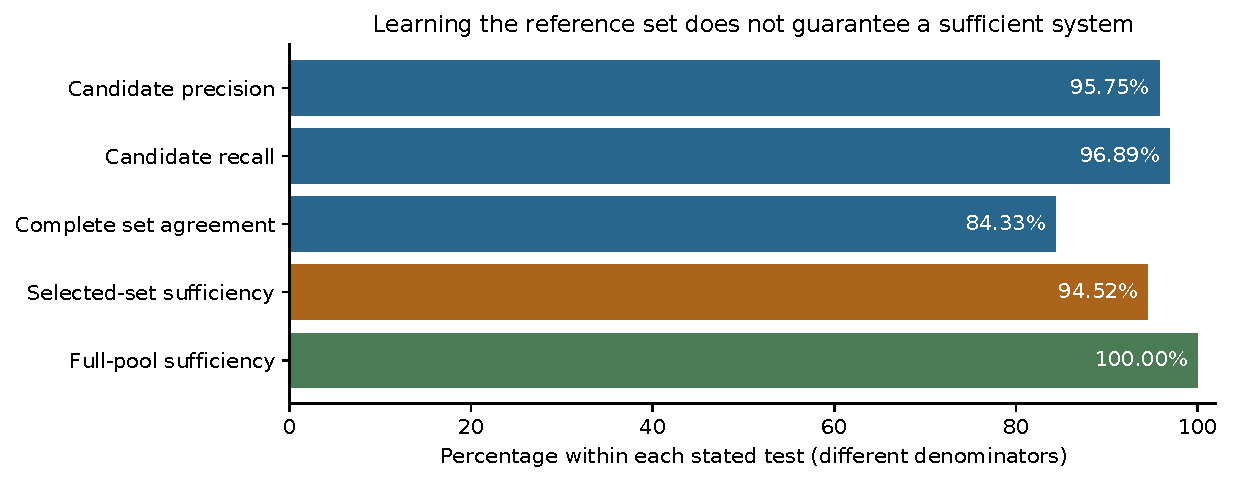
\includegraphics[width=.92\linewidth]{paper_figures/project_labels.pdf}
\caption{The initial seed model learns useful reference sets, but exact sufficiency requires a separate test. All percentages use the frozen model and the 690,382 reserved targets. Label precision and recall count candidates; set agreement and sufficiency count targets. The complete supplied pool resolves every target. These are different measures, not successive stages of one probability.}
\label{fig:project-labels}
\end{figure}
